\chapter{Machine Learning Applications}
\label{sec:chapter_ml}
\begin{refsection}[sections/chapter_ml_references.bib]
\noindent\emph{Editorial note: The six paper summaries identified as source excerpts retain the papers' wording. PDF line wrapping and typographic formatting are normalized. Figure, table and bracketed reference numbers within an excerpt refer to the original paper. Screenshot captions are editorial.}
\medskip

Next-generation wireless networks are increasingly characterized by extreme densification, diverse Quality of Service (QoS) requirements, dynamic topology changes, and highly non-stationary propagation environments. Conventional Medium Access Control (MAC) protocols rely predominantly on static rules, pre-configured backoff parameters, or idealized heuristic policies designed for stationary conditions. Consequently, traditional approaches struggle to adapt in complex, unpredictable scenarios such as industrial automation, massive machine-type communications (mMTC), and high-mobility vehicular swarms.

To address these limitations, machine learning (ML)---particularly Reinforcement Learning (RL) and Multi-Armed Bandit (MAB) frameworks---has emerged as a foundational methodology for intelligent protocol design. By framing radio resource allocation, scheduling, and channel access as learning problems, wireless nodes can autonomously optimize their transmission strategies through continuous interaction with the physical environment. This chapter explores key machine learning applications in modern wireless MAC design, focusing on Phasic Policy Gradient reinforcement learning for Industrial IoT, contextual bandits for 5G New Radio initial access, and deep reinforcement learning for dynamic wireless environments.

% ============================================================
\section{Reinforcement Learning in Wireless Medium Access}
\label{sec:rl_mac_principles}
% ============================================================

\subsection{The Wireless MAC as a Markov Decision Process}
Reinforcement learning operates within the mathematical framework of a Markov Decision Process (MDP), characterized by the tuple $(\mathcal{S}, \mathcal{A}, \mathcal{P}, \mathcal{R}, \gamma)$, where:
\begin{itemize}
    \item $\mathcal{S}$ is the state space representing observable network conditions (e.g., local buffer occupancy, perceived channel interference, recent collision history, and link quality metrics).
    \item $\mathcal{A}$ denotes the action space available to the MAC entity (e.g., contention window size, transmission power level, transmission slot, or carrier frequency).
    \item $\mathcal{P}(s' | s, a) = \mathbb{P}(S_{t+1} = s' | S_t = s, A_t = a)$ defines the transition probability distribution between states under action $a$.
    \item $\mathcal{R}(s, a, s')$ is the reward signal returned by the environment, reflecting key performance indicators such as successful packet delivery, throughput, latency penalty, or energy efficiency.
    \item $\gamma \in [0, 1)$ is the discount factor balancing instantaneous rewards against future expectations.
\end{itemize}

The learning objective is to discover an optimal policy $\pi^*(a | s)$ that maximizes the expected cumulative discounted return:
\begin{equation}
    J(\pi) = \mathbb{E}_{\pi} \left[ \sum_{t=0}^{\infty} \gamma^t R(S_t, A_t, S_{t+1}) \right].
\end{equation}

% ============================================================
\clearpage
\section{Phasic Policy Gradient for Industrial IoT}
\label{sec:ppg_tsch_networks}
\noindent\emph{Selected verbatim excerpts from the paper}~\cite{ml_ppg2022}.

\medskip
\noindent\textbf{Background.}
The devices in IIoT are mostly battery operated and hence cannot afford to keep their radio on for long hours. Hence the transmission, reception and sleep routines of nodes has to be scheduled to save their energy and to provide a synchronized connection in the network. The nodes in TSCH network communicate using a scheduling matrix composed of cells which are designated by its time slot index and the channel index. Recently, learning algorithms such as machine learning (ML) and reinforcement learning (RL) methods are being adopted to address resource allocation problems in wireless networks [2]. Cobbe et al. proposed the PPG, by modifying the traditional actor-critic policy gradient method [3]. In PPG, the policy and the value functions are learnt independently so that the sharing of network parameters between the value optimization and the policy optimization networks can be regulated.

\medskip
\noindent\textbf{Proposed scheme.}
During policy phase, the agent is trained using proximal policy optimization (PPO) [5]. During auxiliary phase, the features from the value function are distilled into the policy network, so that the future policy phases improve.

In auxiliary phase, the joint objective function that includes behavioral cloning loss and an arbitrary auxiliary loss is used to optimized the policy network.

\medskip
\noindent\textbf{Major outcomes.}
We consider that the network consists of 70 nodes communicating to a border router over a maximum of 3 hops. We compare the performance of our proposed scheduling algorithm with that of PPO [5] based algorithm and the Minimum Scheduling Function (MSF) [6], which is a default scheduling algorithm in TSCH networks.

It can be seen that the PPG achieves a better reward than PPO right from the starting of the training phase and converges quickly.

We show that the PPG improves the system throughput by 58\% compared to the default scheduling algorithm MSF and 22\% over the proximal policy optimization method (PPO).

\begin{figure}[H]
\centering
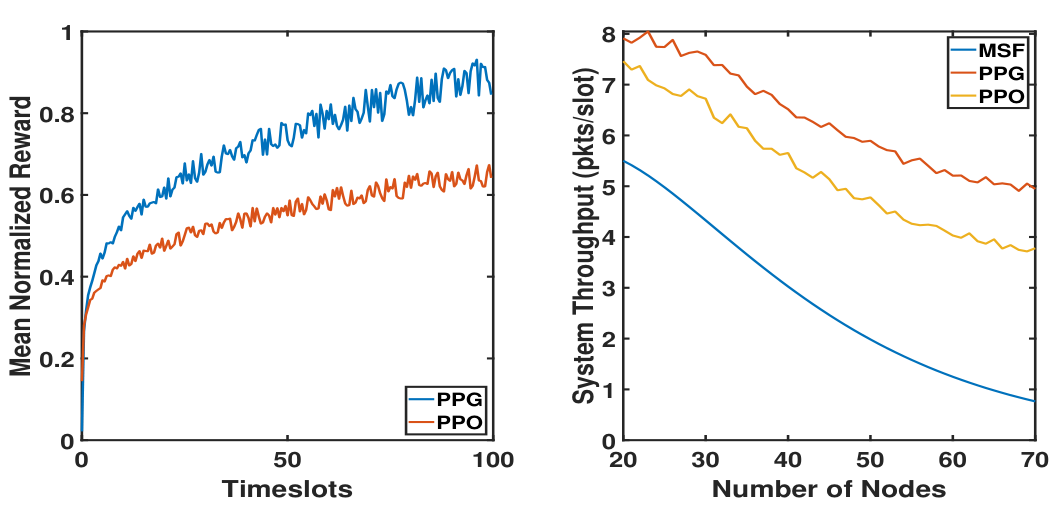
\includegraphics[width=0.76\textwidth,height=4.6cm,keepaspectratio]{ML_chapter_figures/ppg_results.png}
\caption{PPG convergence and system throughput. Screenshot of Fig.~1 in~\cite{ml_ppg2022}.}
\label{fig:ml_ppg_results}
\end{figure}
\clearpage
\section{Contextual Bandits for 5G NR Initial Access}
\label{sec:contextual_bandits_5gnr}
% ============================================================

\subsection{Random Access and Numerology Selection in 5G NR}
Fifth-generation (5G) New Radio (NR) networks support massive Machine-Type Communications (mMTC), where tens of thousands of IoT devices attempt random access over common Random Access Channel (RACH) occasions. In the millimeter-wave (mmWave) spectrum, directional beamforming and severe sensitivity to physical blockages (e.g., humans, vehicles, foliage) exacerbate initial access latency.

To accommodate heterogeneous services and diverse channel conditions, 5G NR introduces \emph{flexible numerology}, where subcarrier spacing (SCS) $\Delta f$ is scalable according to:
\begin{equation}
    \Delta f = 2^\mu \times 15~\text{kHz}, \quad \mu \in \{0, 1, 2, 3, 4\}.
\end{equation}
Different numerologies offer distinct trade-offs: smaller SCS ($\mu = 0, 1$) provides longer symbol duration and robust cyclic prefix protection against delay spread, whereas larger SCS ($\mu = 2, 3$) shortens slot duration, reducing RACH occasion latency and mitigating Doppler shift at the expense of higher sensitivity to phase noise and inter-carrier interference.

\subsection{Contextual Multi-Armed Bandit Formulation}
Choosing the optimal numerology $\mu$ dynamically cannot rely on slow feedback loops during initial access because the device has not yet established radio resource control (RRC) connectivity. Bommisetty and Venkatesh formulated this problem as a \emph{Contextual Multi-Armed Bandit} (CMAB).

In the CMAB framework:
\begin{itemize}
    \item At decision round $t$, the base station observes a contextual vector $\mathbf{x}_t \in \mathbb{R}^d$ summarizing environmental states, such as spatial blockage density, user mobility indicators, and aggregate channel busy ratios.
    \item The agent selects an arm $a_t \in \mathcal{A} = \{\mu_0, \mu_1, \dots, \mu_K\}$, representing the active numerology configuration for the upcoming RACH slot.
    \item The network executes initial access and receives a scalar reward $r_{t, a_t}$, proportional to the number of successfully connected devices and inversely proportional to connection latency.
\end{itemize}

\subsection{Upper Confidence Bound (UCB) Action Selection}
To balance exploration of unverified numerologies against exploitation of proven configurations, the agent employs the contextual Upper Confidence Bound (LinUCB) policy:
\begin{equation}
    a_t = \arg\max_{a \in \mathcal{A}} \left[ \mathbf{x}_t^T \hat{\boldsymbol{\theta}}_a + \alpha \sqrt{\mathbf{x}_t^T \mathbf{A}_a^{-1} \mathbf{x}_t} \right],
\end{equation}
where $\hat{\boldsymbol{\theta}}_a = \mathbf{A}_a^{-1} \mathbf{b}_a$ is the ridge-regression weight vector estimate for arm $a$, $\mathbf{A}_a = \mathbf{I}_d + \sum_{\tau \in \mathcal{T}_a} \mathbf{x}_\tau \mathbf{x}_\tau^T$ is the covariance matrix, and $\alpha > 0$ controls the confidence exploration width.

By adapting numerology to real-time blockage context, the contextual bandit mechanism increases successful device connections by over $40\%$ per RACH occasion compared to static numerology schemes, substantially reducing network access delay in high-density mMTC deployments.

% ============================================================
\section{Deep Reinforcement Learning in Dynamic Wireless Environments}
\label{sec:drl_dynamic_wireless}
% ============================================================

Beyond scheduling and initial access, Deep Reinforcement Learning (DRL) algorithms (including Deep Q-Networks and Double Deep Q-Networks with prioritized experience replay) are widely deployed across wireless protocol stacks:
\begin{itemize}
    \item \textbf{Dynamic Rate and Power Adaptation:} In fast-fading vehicular and mobile environments, DRL agents learn joint modulation, coding, and power adaptation policies directly from raw signal-to-noise ratio trajectories without requiring explicit channel state information (CSI) models.
    \item \textbf{Cognitive Spectrum Sharing:} In multi-tier heterogeneous networks, secondary users employ actor-critic policies to identify idle spectral white spaces and adjust transmission parameters without causing harmful interference to primary licensees.
    \item \textbf{Integrated Sensing and Communication (ISAC):} DRL facilitates the joint optimization of radar sensing beams and communication data streams in connected vehicular environments, enabling reliable situational awareness and high-throughput infotainment.
\end{itemize}

Through modern reinforcement learning and bandit algorithms, wireless MAC protocols transition from rigid, handcrafted heuristics to intelligent, self-optimizing architectures capable of delivering robust performance across diverse 5G-Advanced and 6G communication environments.

\clearpage
\section{DQN-Based Joint Scheduling of eMBB and Massive URLLC}
\label{sec:ml_dqn_joint}
\noindent\emph{Selected verbatim excerpts from the paper}~\cite{ml_dqn2025}.

\medskip
\noindent\textbf{Background.}
In 5G, the most popular approach to accomodate low latency users in the same network is through puncturing. The high data rate eMBB users are punctured and a minislot worth of resource is used by URLLC user.

The punctured EMBB users experience a degradation in reliability [14]. As more resource blocks are punctured, the error probability in decoding the block becomes difficult.

\medskip
\noindent\textbf{Proposed scheme.}
To circumvent this, we introduce a hybrid scheme that switches to orthogonal multiplexing mode for a fixed number of RBs and puncturing mode for the rest of the RBs whenever the URLLC arrival rate shoots up.

Let K be the number of RBs dedicated to URLLC data and N be the total number of resource blocks in a minislot.

\medskip
\noindent\textbf{Major outcomes.}
The results highlight that the baseline puncturing strategy experiences performance degradation much earlier under increasing traffic load. In contrast, the DQN agent maintains superior performance by dynamically adapting its actions at each time slot, effectively addressing the reliability demands of both URLLC and eMBB services. However, even the DQN approach reaches a saturation point at very high arrival rates, constrained by the system's total available bandwidth and throughput.

The DQN-based approach consistently outperforms the baseline, keeping latency significantly lower across all $\lambda_u$. While the baseline exhibits a sharp increase in delay---exceeding 8 ms under high traffic---the DQN model effectively mitigates queue build-up through dynamic resource adaptation.

\begin{figure}[H]
\centering
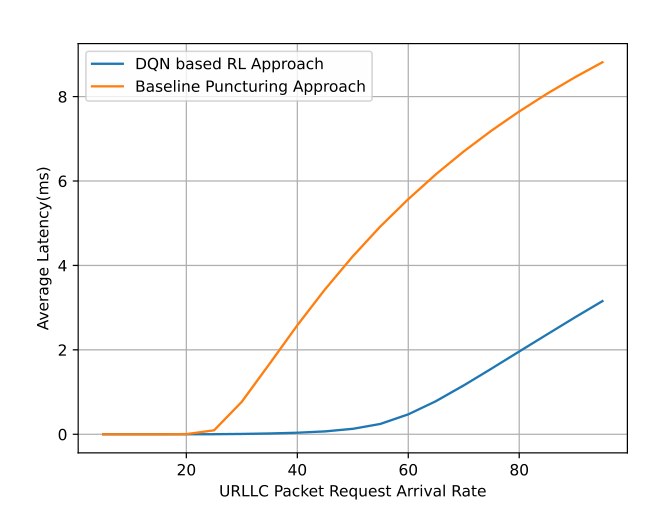
\includegraphics[width=0.49\textwidth,height=4.6cm,keepaspectratio]{ML_chapter_figures/dqn_latency.png}
\caption{Average URLLC latency. Screenshot of Fig.~6 in~\cite{ml_dqn2025}.}
\label{fig:ml_dqn_latency}
\end{figure}
\clearpage
\section{Intrusion Detection with Efficient Feature Selection}
\label{sec:ml_feature_selection}
\noindent\emph{Selected verbatim excerpts from the paper}~\cite{ml_features2023}.

\medskip
\noindent\textbf{Background.}
The primary features are insufficient to predict the network attacks with very high precision. Derived features are generated by applying some statistical functions or transformations to the primary features. These derived features give us greater insight into the behavior of the network in case of an attack. ASNM dataset provides a large set of derived features. Generating a large number of derived features increases the complexity of the model. Hence feature selection techniques become important.

\medskip
\noindent\textbf{Proposed scheme.}
We apply Chi-squared Test feature selection technique on the Advanced Security Network Metrics dataset to choose highly dependent features and remove features independent of the classifier output.

We build a Logistic Regression based and a Neural Network based IDS on this dataset and obtain a highly accurate Network attack detection model.

We perform a 5-fold cross validation on all the three datasets, where each dataset is split into 5 stratified sets and the mean of the individual performance metrics are recorded.

\medskip
\noindent\textbf{Major outcomes.}
After use of Chi-squared test, we obtain a good performance result and the classifier trains much faster. The number of nodes in the input layer reduces, so the number of computations also reduces greatly.

Flow based features and their derived features give us better performance over the primary features, but the flow based features have a larger memory footprint. Feature Selection methods in combination with Deep Learning algorithms is one of the best solutions to intrusion detection systems. We can compromise on number of features in case of timing constraints.

\begin{figure}[H]
\centering
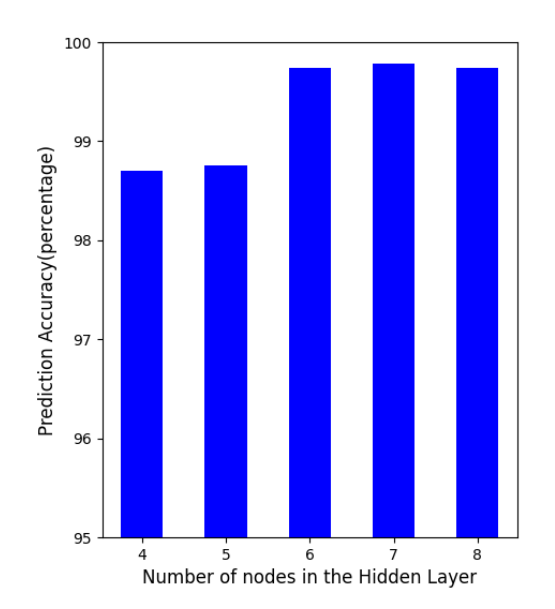
\includegraphics[width=0.44\textwidth,height=4.5cm,keepaspectratio]{ML_chapter_figures/ids_feature_selection.png}
\caption{Selection of hidden-layer size. Screenshot of Fig.~2 in~\cite{ml_features2023}.}
\label{fig:ml_ids_feature_selection}
\end{figure}
\clearpage
\section{Hybrid Deep Models for Automatic Modulation Classification}
\label{sec:ml_amc}
\noindent\emph{Selected verbatim excerpts from the paper}~\cite{ml_amc2024}.

\medskip
\noindent\textbf{Background.}
Automatic Modulation Classification (AMC) plays a pivotal role in modern wireless communication systems, enabling receivers to autonomously identify modulation schemes without requiring prior knowledge of the transmitter's settings. This capability is essential for enhancing the efficiency, robustness, and adaptability of real-time applications such as 5G networks, dynamic spectrum allocation, and interference mitigation.

\medskip
\noindent\textbf{Proposed scheme.}
The Hybrid 1 model integrates the strengths of the RanNet and VGG architectures to create a novel hybrid approach. The core idea is to enhance the feature extraction capabilities of RanNet by incorporating additional layers from VGG. Specifically, a convolutional layer with a maxpooling layer and a skip connection is added between the two Ranblocks, aimed at retaining critical information during initial processing.

Inspired by the Chain Residual Pooling block from RefineNet, the X block improves the model's ability to capture contextual information from large input regions.

In this architecture, two Ranblocks are employed, each incorporating an X block in place of the traditional Feablock.

\medskip
\noindent\textbf{Major outcomes.}
At an SNR of 18 dB, the Hybrid 2 model achieves an accuracy of 87.69\%, as shown in Fig. 10.

The comparison shows that Hybrid 1 and Hybrid 2 models achieve higher classification accuracies at most SNR levels, with Hybrid 1 slightly outperforming Hybrid 2 at very low SNR values. Hybrid 3, while still competitive, demonstrates lower accuracy, indicating that the architectural enhancements in Hybrid 1 and Hybrid 2 are more effective in improving classification performance.

\begin{figure}[H]
\centering
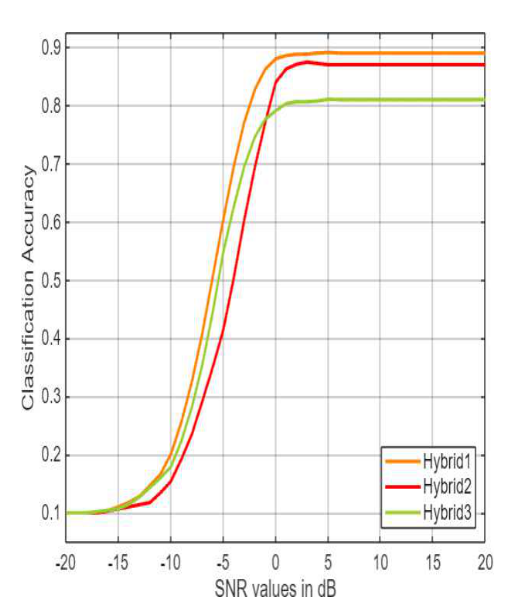
\includegraphics[width=0.43\textwidth,height=4.6cm,keepaspectratio]{ML_chapter_figures/amc_hybrid_comparison.png}
\caption{Comparison of hybrid architectures. Screenshot of Fig.~17 in~\cite{ml_amc2024}.}
\label{fig:ml_amc_hybrid_comparison}
\end{figure}
\clearpage
\section{Robust Intrusion Detection for Previously Unseen Attacks}
\label{sec:ml_rnids}
\noindent\emph{Selected verbatim excerpts from the paper}~\cite{ml_rnids2022}.

\medskip
\noindent\textbf{Background.}
However, whether an ML-based NIDS can successfully handle a new type of attack is an open question. CNN-based IDS can classify these types of attacks to a certain extent but they classify most unknown attacks as benign. Due to this problem, a robust outlier detection in the NIDS system becomes necessary. The purpose of this paper is to address this vital issue.

\medskip
\noindent\textbf{Proposed scheme.}
We put forward a Robust NIDS model, called RNIDS, which is a combination of CNN followed by an outlier detection system. The combined system classifies known attacks and identifies new outliers with high accuracy.

We further analyze the prediction probabilities of the neural network using nearest neighbor approximation. This information helps us decide if a new adversary was attempting a malicious attack on the network.

If the average distance is beyond a certain threshold dth, then the point is classified as a new adversary.

\medskip
\noindent\textbf{Major outcomes.}
The CNN model with 13 attack classes has classified different attacks with an overall accuracy of 98.3\%.

Compared to the results in Table V, Botnet, Port scan and SSH Patator are predicted as a new adversary with an accuracy of 74.96\%, 88.03\% and 90.08\%.

Retraining the CNN model with an appropriate balance of initial dataset and real time data will be a difficult task. There is a high chance that the CNN may forget the patterns from the initial data if we feed it a large set of newer samples.

\begin{figure}[H]
\centering
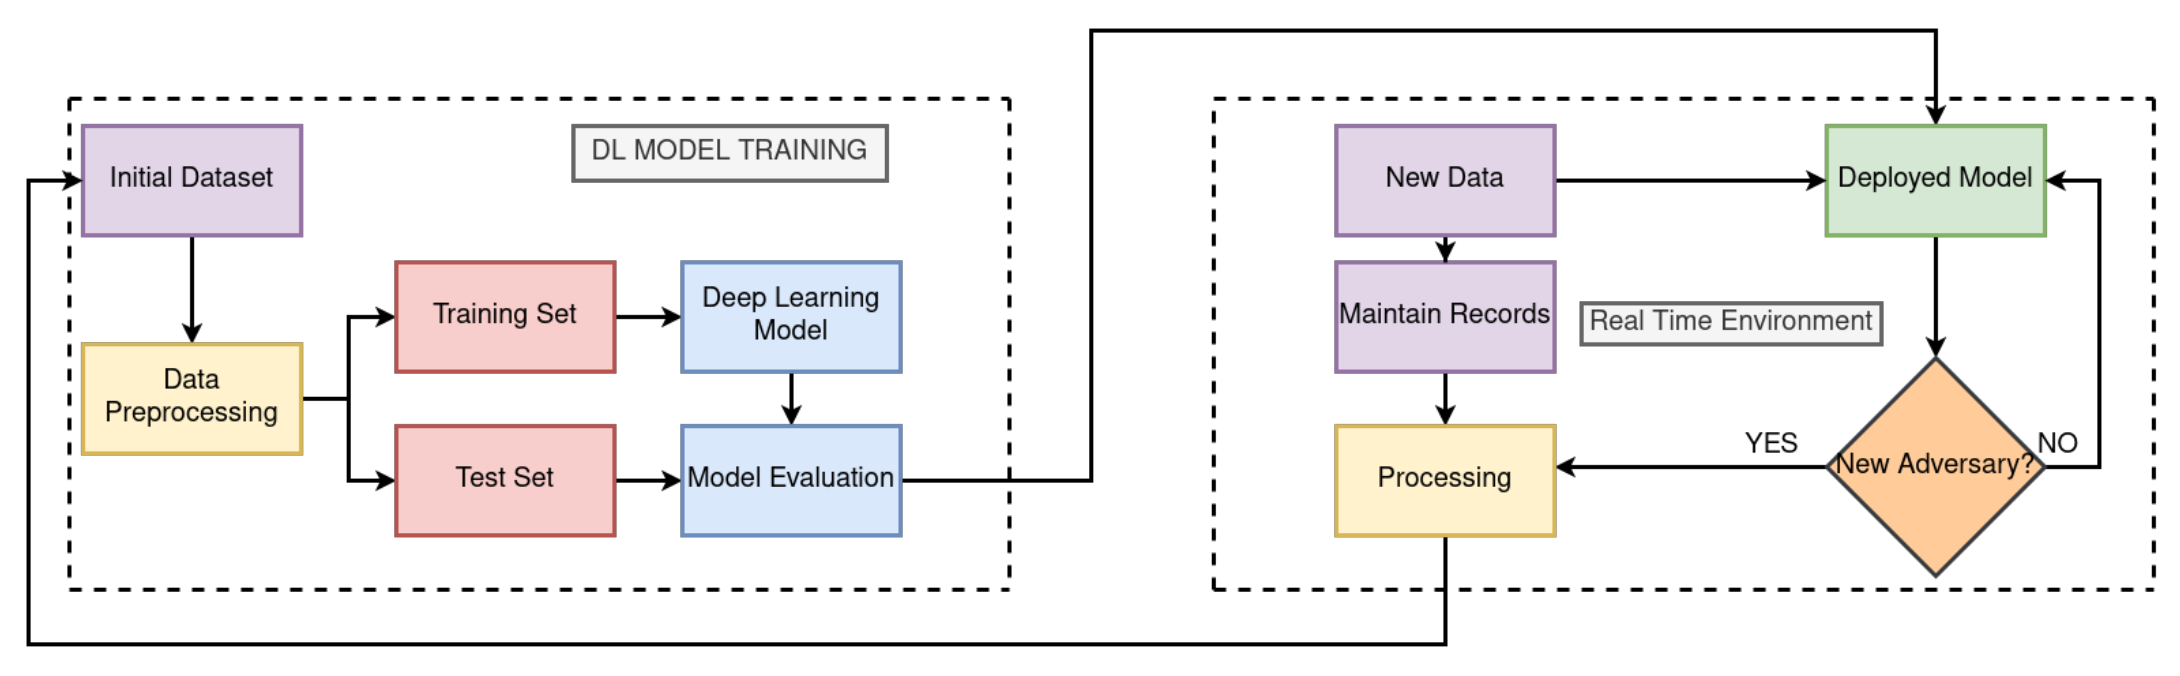
\includegraphics[width=0.96\textwidth,height=4.5cm,keepaspectratio]{ML_chapter_figures/rnids_architecture.png}
\caption{RNIDS training and deployment. Screenshot of Fig.~1 in~\cite{ml_rnids2022}.}
\label{fig:ml_rnids_architecture}
\end{figure}
\clearpage
\section{BIOS: Biogeography-Inspired Scheduling for TSCH}
\label{sec:ml_bios}
\noindent\emph{Selected verbatim excerpts from the paper}~\cite{ml_bios2021}.

\medskip
\noindent\textbf{Background.}
The devices in IIoT are mostly battery operated and hence cannot afford to keep their radio on for long hours.

In TSCH, the time is divided into slots and the bandwidth is divided into orthogonal channels [4]. The nodes in TSCH network communicate in a scheduling matrix composed of cells. The cells are the basic resource units for communication in TSCH network which are designated by its time slot index and the channel index.

IEEE 802.15.4e standard does not define the algorithm for computing the scheduling matrix and is open to implementation. Hence the problem of designing efficient schedule in TSCH networks has gained importance in networking research community.

\medskip
\noindent\textbf{Proposed scheme.}
In initiation stage, a set of random schedules are generated. To improve the existing set of scheduling algorithms, we employ the migration and mutation operations. Migration operation shares the good features from best scheduling algorithm to the poor ones by appropriately modelling the immigration and emigration of each node in the network. Mutation operation maintains the diversity in the candidate schedules to tackle the sporadic changes in the network.

\medskip
\noindent\textbf{Major outcomes.}
It has been shown through simulations that the proposed BIOS scheduling algorithm achieves an improvement of 60\% in delay performance and upto 40\% of energy efficiency compared to MSF.

In the mobile TSCH networks, the topology changes frequently forcing BIOS to explore more solutions by mutation operation which makes the solution convergence slower.

\begin{figure}[H]
\centering
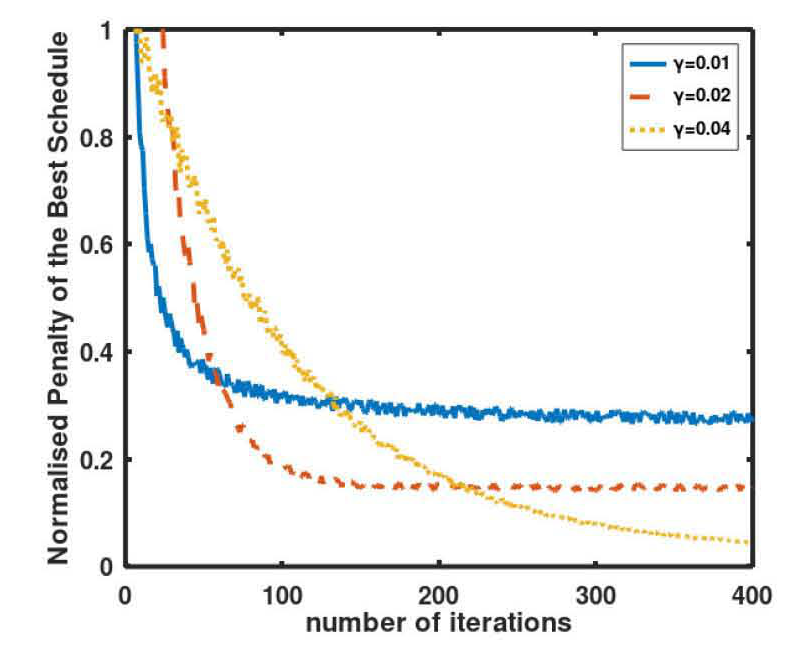
\includegraphics[width=0.48\textwidth,height=4.5cm,keepaspectratio]{ML_chapter_figures/bios_mobile_convergence.png}
\caption{BIOS convergence with mobile nodes. Screenshot of Fig.~3 in~\cite{ml_bios2021}.}
\label{fig:ml_bios_mobile_convergence}
\end{figure}
\clearpage
\printbibliography[heading=subbibliography,title={References for the Paper Summaries}]
\end{refsection}
